\documentclass[10pt]{article}

\usepackage[utf8]{inputenc}
\usepackage[spanish]{babel}
\decimalpoint

\usepackage{csquotes}
\usepackage[T1]{fontenc}
\usepackage{lmodern}
\usepackage[a4paper, total={6.7in, 11in}]{geometry}
\usepackage{amsmath}
\usepackage{amssymb}
\usepackage[per-mode=fraction, inter-unit-product=\cdot, quotient-mode=fraction]{siunitx}
\usepackage{float}
\usepackage{hyperref}
\usepackage{xcolor}
\usepackage{tablefootnote}
\usepackage{chemformula}

\usepackage[shortlabels]{enumitem}
\setlist{listparindent=\parindent}

\usepackage{tikz}
\usetikzlibrary{babel}
\usetikzlibrary{patterns}
\allowdisplaybreaks

\newcommand{\comment}[1]{\text{\phantom{(#1)}} \tag{#1}}
\newcommand*\diff{\mathop{}\!\mathrm{d}}
\newcommand{\inv}[1]{\frac{1}{#1}}
\newcommand{\deriv}[2]{\dfrac{\diff #1}{\diff #2}}
\newcommand{\ROM}[1]{%
  \textup{\uppercase\expandafter{\romannumeral#1}}%
}

\usepackage{graphicx}
\graphicspath{{./}}

\begin{document}

\begin{table}
	\centering
	\begin{tabular}{|p{4cm}|l|l|}
		\hline
		Propiedad                                                                                                                                                                 & NMOS                                                                                              & PMOS                                                                         \\
		\hline
		                                                                                                                                                                          &                                                                                                   &                                                                              \\
		\textbf{Tensión de \textit{overdrive}}                                                                                                                                    & $V_{OV} = V_{GS} - V_{TH}$                                                                        & $V_{OV} = V_{SG} - |V_{TH}|$                                                 \\
		                                                                                                                                                                          &                                                                                                   &                                                                              \\
		\hline
		                                                                                                                                                                          &                                                                                                   &                                                                              \\
		\textbf{Subumbral}                                                                                                                                                        & $V_{GS} < V_{TH}$                                                                                 & $V_{SG} < |V_{TH}|$                                                          \\
		                                                                                                                                                                          & $I_D = I_{D_0}\exp\left(\dfrac{V_{GS} - V_{TH}}{S}\ln10\right)$                                   & $I_D = I_{D_0}\exp\left(\dfrac{V_{SG} - |V_{TH}|}{S}\ln10\right)$            \\
		                                                                                                                                                                          &                                                                                                   &                                                                              \\
		\hline
		                                                                                                                                                                          & \multicolumn{2}{|c|}{}                                                                                                                                                           \\
		\textbf{Límite de subumbral}                                                                                                                                              & \multicolumn{2}{|c|}{$I_{D_0} = I_D(V_{OV} = 0) \approx \SI{0.1}{\micro\ampere}\cdot\frac{W}{L}$}                                                                                \\
		                                                                                                                                                                          & \multicolumn{2}{|c|}{}                                                                                                                                                           \\
		\hline
		                                                                                                                                                                          &                                                                                                   &                                                                              \\
		\textbf{Triodo}                                                                                                                                                           & $V_{DS} < V_{GS} - V_{TH} \land V_{GS} > V_{TH}$                                                  & $V_{SD} < V_{SG} - |V_{TH}| \land V_{SG} > |V_{TH}|$                         \\
		                                                                                                                                                                          & $I_D = K\left[(V_{GS} - V_{TH})V_{DS} - \frac{1}{2}V_{DS}^2\right]$                               & $I_D = K\left[(V_{SG} - |V_{TH}|)V_{SD} - \frac{1}{2}V_{SD}^2\right]$        \\
		                                                                                                                                                                          &                                                                                                   &                                                                              \\
		\hline
		                                                                                                                                                                          &                                                                                                   &                                                                              \\
		\textbf{Resistencia de canal en triodo} [\si{\ohm}]                                                                                                                       & $R_{ch} = \dfrac{V_{DS}}{I_D} = \dfrac{1}{K(V_{GS} - V_{TH})}$                                    & $R_{ch} = \dfrac{V_{SD}}{I_D} = \dfrac{1}{K(V_{SG} - |V_{TH}|)}$             \\
		                                                                                                                                                                          &                                                                                                   &                                                                              \\
		\hline
		                                                                                                                                                                          &                                                                                                   &                                                                              \\
		\textbf{Saturación}                                                                                                                                                       & $V_{DS} > V_{GS} - V_{TH} \land V_{GS} > V_{TH}$                                                  & $V_{SD} > V_{SG} - |V_{TH}| \land V_{SG} > |V_{TH}|$                         \\
		                                                                                                                                                                          & $I_D = \frac{1}{2}K(V_{GS} - V_{TH})^2$\color{red}{$(1 + \lambda V_{DS})$}                        & $I_D = \frac{1}{2}K(V_{SG} - |V_{TH}|)^2$\color{red}{$(1 - \lambda V_{SD})$} \\
		                                                                                                                                                                          &                                                                                                   &                                                                              \\
		\hline
		\textbf{Transconductancia}\tablefootnote{Con dos de tres de $I_D$, $V_{OV}$ y $\frac{W}{L}$ se puede determinar la variable faltante al pasar por $g_m$.} [\si{\siemens}] &
		{\begin{minipage}{0cm}
					 \begin{align*}
						g_m & = \left.\frac{\partial I_D}{\partial V_{GS}}\right\vert_Q \\
						g_m & = K(V_{GS} - V_{TH})                                      \\
						g_m & = \frac{2I_D}{V_{GS} - V_{TH}}                            \\
						g_m & = \sqrt{2KI_D}
					\end{align*}
				 \end{minipage}}                                                                                                                                                 &
		{\begin{minipage}{0cm}
					 \begin{align*}
						g_m & = \left.\dfrac{\partial I_D}{\partial V_{SG}}\right\vert_Q \\
						g_m & = K(V_{SG} - |V_{TH}|)                                     \\
						g_m & = \frac{2I_D}{V_{SG} - |V_{TH}|}                           \\
						g_m & = \sqrt{2KI_D}
					\end{align*}
				 \end{minipage}}                                                                                                                                                                                                                                                                                                                                    \\
		                                                                                                                                                                          &                                                                                                   &                                                                              \\
		\hline
	\end{tabular}
	\caption{Transistores MOSFET}
\end{table}

\begin{table}[h]
	\centering
	\begin{tabular}{|l|c|c|c|}
		\hline
		Región de operación & $C_{GD}$            & $C_{GB}$ & $C_{GS}$            \\
		\hline
		                    &                     &          &                     \\
		Subumbral           & $C_{OV}$            & $C_{OX}$ & $C_{OV}$            \\
		                    &                     &          &                     \\
		\hline
		                    &                     &          &                     \\
		Triodo              & $\frac{1}{2}C_{OX}$ & $C_{OX}$ & $\frac{1}{2}C_{OX}$ \\
		                    &                     &          &                     \\
		\hline
		                    &                     &          &                     \\
		Saturación          & $C_{OV}$            & $C_{OX}$ & $\frac{2}{3}C_{OX}$ \\
		                    &                     &          &                     \\
		\hline
	\end{tabular}
	\caption{Capacitancias parásitas}
\end{table}

\begin{table}
	\centering
	\begin{tabular}{|l|l|}
		\hline
		                                                     &                                                          \\
		\textbf{Permitividad del vacío}                      & $\varepsilon_0 = \SI{8.854e-14}{\farad\per\centi\meter}$ \\
		                                                     &                                                          \\
		\hline
		                                                     &                                                          \\
		\textbf{Permitividad relativa del \ch{SiO2}}         & $\varepsilon_{ox} = \num{3.9}$                           \\
		                                                     &                                                          \\
		\hline
		                                                     &                                                          \\
		\textbf{Voltaje térmico a \SI{300}{K}}               & $V_t = \SI{26}{mV}$                                      \\
		                                                     &                                                          \\
		\hline
		                                                     &                                                          \\
		\textbf{Pendiente de subumbral a \SI{300}{K}}        & $S \approx \SI{60}{mV/déc}$                              \\
		                                                     &                                                          \\
		\hline
		                                                     &                                                          \\
		\textbf{Pendiente de subumbral a \SI{100}{\celsius}} & $S \approx \SI{80}{mV/déc}$                              \\
		                                                     &                                                          \\
		\hline
	\end{tabular}
	\caption{Constantes}
\end{table}

\begin{table}
	\centering
	\begin{tabular}{|p{5cm}|l|}
		\hline
		Parámetro                                                                                                                                                                                                                                                                                    & Expresión                                                                                                                             \\
		\hline
		                                                                                                                                                                                                                                                                                             &                                                                                                                                       \\
		\textbf{Tensión de \textit{flatband}} [\si{\volt}]                                                                                                                                                                                                                                           & $V_{FB} = \phi_B = 2\phi_S = V_t \ln\left(\dfrac{N_A}{N_i}\right)$                                                                    \\
		                                                                                                                                                                                                                                                                                             &                                                                                                                                       \\
		\hline
		                                                                                                                                                                                                                                                                                             &                                                                                                                                       \\
		\textbf{Tensión de umbral con efecto de sustrato}\tablefootnote{Lo de $\sqrt{\si{V}}$ viola el SI y por tanto no puede ser evaluado en \texttt{units}. Montero mamó mientras explicaba esto, signos y valores absolutos podrían estar mal. El Razavi tampoco lo explica mucho.} [\si{\volt}] & $V_{TH} = V_{TH_0} + \gamma\left(\sqrt{\left|2V_{FB} + V_{SB}\right|} - \sqrt{2V_{FB}}\right)$                                        \\
		                                                                                                                                                                                                                                                                                             &                                                                                                                                       \\
		\hline
		                                                                                                                                                                                                                                                                                             &                                                                                                                                       \\
		\textbf{Resistencia de pequeña señal con $\lambda \ne 0$} [\si{\ohm}]                                                                                                                                                                                                                        & $r_o = \dfrac{1}{\lambda I_D}$                                                                                                        \\
		                                                                                                                                                                                                                                                                                             &                                                                                                                                       \\
		\hline
		                                                                                                                                                                                                                                                                                             &                                                                                                                                       \\
		\textbf{Ganancia} [\si{\volt/\volt}]                                                                                                                                                                                                                                                         & $A_v = \dfrac{v_{out}}{v_{in}}$                                                                                                       \\
		                                                                                                                                                                                                                                                                                             &                                                                                                                                       \\
		\hline
		                                                                                                                                                                                                                                                                                             &                                                                                                                                       \\
		\textbf{Pendiente de subumbral} [mV/década]                                                                                                                                                                                                                                                  & $S = \left[\dfrac{\diff}{\diff V_{GS}}\log I_{DS}\right]^{-1} = (\ln 10)V_t\,m = (\ln 10)V_t\left(1 + \dfrac{C_{dep}}{C_{ox}}\right)$ \\
		                                                                                                                                                                                                                                                                                             &                                                                                                                                       \\
		\hline
		                                                                                                                                                                                                                                                                                             &                                                                                                                                       \\
		\textbf{Longitud efectiva de canal}\tablefootnote{Cuando esto ocurre, $L = L_\text{eff}$ en todo lado.} [\si{\centi\meter}]                                                                                                                                                                  & $L_{\text{eff}} = L - 2\Delta L$                                                                                                      \\
		                                                                                                                                                                                                                                                                                             &                                                                                                                                       \\
		\hline
		                                                                                                                                                                                                                                                                                             &                                                                                                                                       \\
		\textbf{Capacitancia del óxido} [\si{\farad\per\centi\meter^2}]                                                                                                                                                                                                                              & $C'_{ox} = \dfrac{\varepsilon_0\varepsilon_{ox}}{t_{ox}}$                                                                             \\
		                                                                                                                                                                                                                                                                                             &                                                                                                                                       \\
		\hline
		                                                                                                                                                                                                                                                                                             &                                                                                                                                       \\
		\textbf{Capacitancia del óxido} [\si{\farad}]                                                                                                                                                                                                                                                & $C_{ox} = C'_{ox}WL$                                                                                                                  \\
		                                                                                                                                                                                                                                                                                             &                                                                                                                                       \\
		\hline
		                                                                                                                                                                                                                                                                                             &                                                                                                                                       \\
		\textbf{Parámetro del proceso} [\si{\ampere\per\volt^2}]                                                                                                                                                                                                                                     & $K' = \mu_n C'_{ox}$                                                                                                                  \\
		                                                                                                                                                                                                                                                                                             &                                                                                                                                       \\
		\hline
		                                                                                                                                                                                                                                                                                             &                                                                                                                                       \\
		\textbf{Transconductancia del proceso} [\si{\ampere\per\volt^2}]                                                                                                                                                                                                                             & $K = \frac{W}{L}K'$                                                                                                                   \\
		                                                                                                                                                                                                                                                                                             &                                                                                                                                       \\
		\hline
	\end{tabular}
	\caption{Parámetros}
\end{table}

\begin{table}
	\centering
	\begin{tabular}{|p{3cm}|c|c|c|}
		\hline
		Propiedad                                  & Common source\tablefootnote{Los valores sin carga se obtienen con $\lim_{R_L\to\infty}{R\parallel R_L} = R$. Montero se voló la fuente de corriente pero no quedó una imagen apropiada para copiar.} & Common gate                           & Common drain                                       \\
		\hline
		                                           &                                                                                                                                                                                                      &                                       &                                                    \\
		\textbf{Caso estudiado}
		                                           & 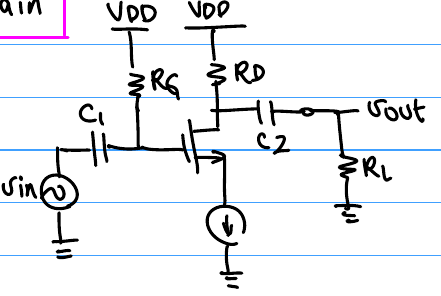
\includegraphics[width=0.20\textwidth, keepaspectratio]{cs}
		                                           & 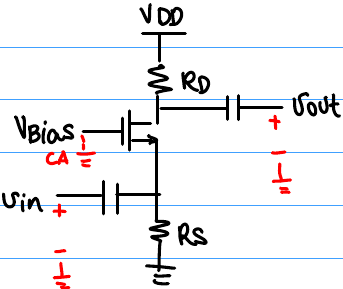
\includegraphics[width=0.20\textwidth, keepaspectratio]{cg}
		                                           & 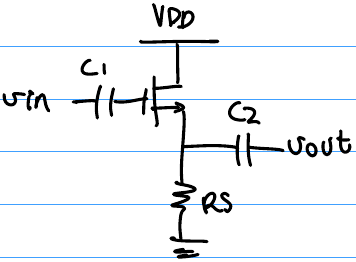
\includegraphics[width=0.20\textwidth, keepaspectratio]{cd}                                                                                                                                                                                                                                       \\
		                                           &                                                                                                                                                                                                      &                                       &                                                    \\
		\hline
		                                           &                                                                                                                                                                                                      &                                       &                                                    \\
		\textbf{Ganancia} [\si{\volt/\volt}]       & $A_v = -g_m(R_D\parallel R_L)$                                                                                                                                                                       & $A_v = g_mR_D$                        & $A_v = \dfrac{R_S}{\frac{1}{g_m} + R_S} \approx 1$ \\
		                                           &                                                                                                                                                                                                      &                                       &                                                    \\
		\hline
		                                           &                                                                                                                                                                                                      &                                       &                                                    \\
		\textbf{Impedancia de entrada} [\si{\ohm}] & $R_{in} = R_G$                                                                                                                                                                                       & $R_{in} = \frac{1}{g_m}\parallel R_S$ & $R_{in} = \infty$                                  \\
		                                           &                                                                                                                                                                                                      &                                       &                                                    \\
		\hline
		                                           &                                                                                                                                                                                                      &                                       &                                                    \\
		\textbf{Impedancia de salida} [\si{\ohm}]  & $R_{out} = R_D\parallel R_L$                                                                                                                                                                         & $R_{out} = R_D$                       & $R_{out} = R_S\parallel\frac{1}{g_m}$              \\
		                                           &                                                                                                                                                                                                      &                                       &                                                    \\
		\hline
	\end{tabular}
	\caption{Topologías de amplificadores}
\end{table}

\begin{table}
	\centering
	\begin{tabular}{|p{0.25\textwidth}|p{0.25\textwidth}|p{0.25\textwidth}|}
		\hline
		                                                                                                &                                                                                                                       \\
		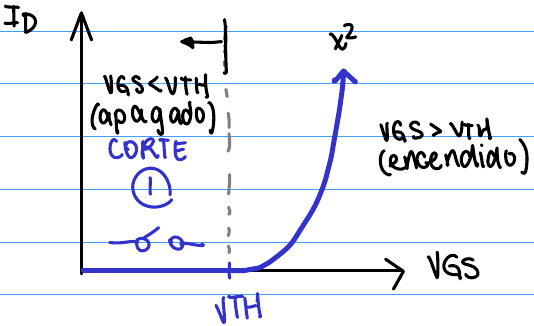
\includegraphics[width=0.25\textwidth, keepaspectratio]{transfer}
		                                                                                                & 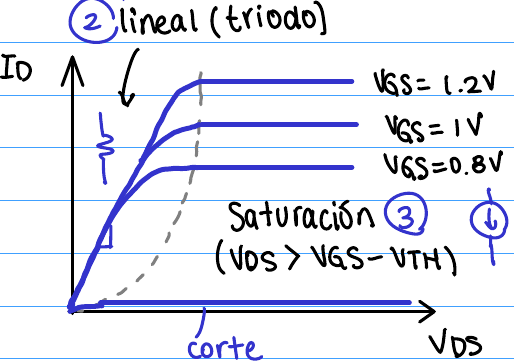
\includegraphics[width=0.25\textwidth, keepaspectratio]{output}
		                                                                                                & 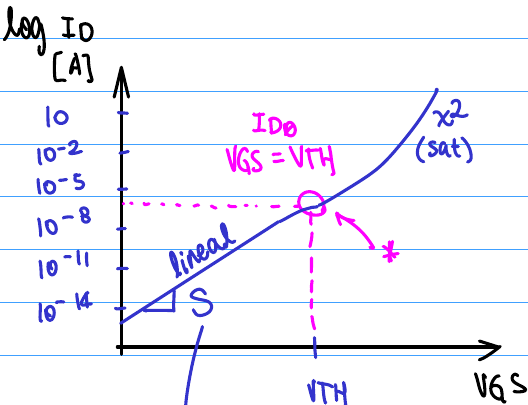
\includegraphics[width=0.25\textwidth, keepaspectratio]{subthreshold}                                                 \\
		Curva de transferencia                                                                          & Curva de salida\tablefootnote{En región lineal el canal es continuo. En saturación se acorta.} & Región de subumbral  \\
		                                                                                                &                                                                                                                       \\
		\hline
		                                                                                                &                                                                                                                       \\
		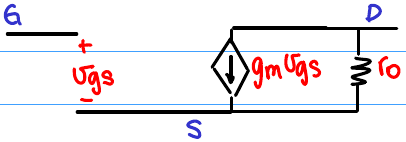
\includegraphics[width=0.25\textwidth, keepaspectratio]{smallsignal-nmos}
		                                                                                                & 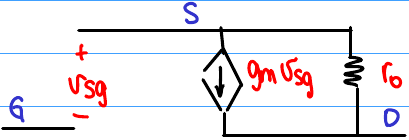
\includegraphics[width=0.25\textwidth, keepaspectratio]{smallsignal-pmos}
		                                                                                                & 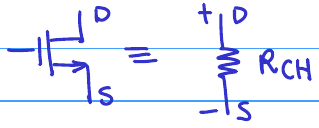
\includegraphics[width=0.25\textwidth, keepaspectratio]{smallsignal-triode}                                           \\
		Modelo de pequeña señal NMOS\tablefootnote{$g_m = \frac{i_d}{v_{gs}} \implies i_d = g_mv_{gs}$} & Modelo de pequeña señal PMOS                                                                   & Modelo de triodo     \\
		                                                                                                &                                                                                                                       \\
		\hline
		                                                                                                &                                                                                                                       \\
		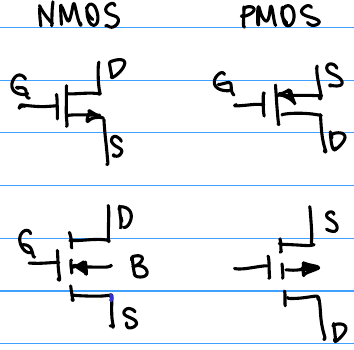
\includegraphics[width=0.25\textwidth, keepaspectratio]{symbols}
		                                                                                                & 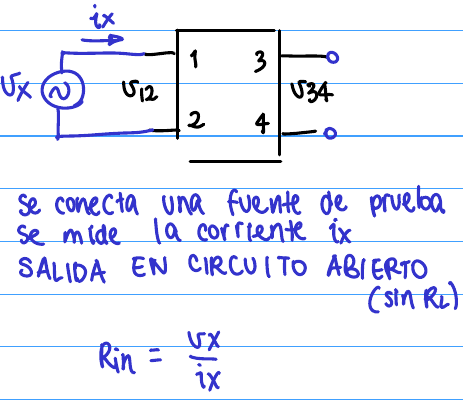
\includegraphics[width=0.25\textwidth, keepaspectratio]{input-impedance}
		                                                                                                & 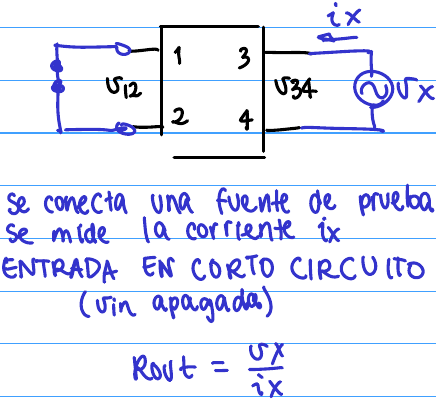
\includegraphics[width=0.25\textwidth, keepaspectratio]{output-impedance}                                             \\
		Simbología                                                                                      & Impedancia de entrada                                                                          & Impedancia de salida \\
		                                                                                                &                                                                                                                       \\
		\hline
	\end{tabular}
	\caption{Gráficas y modelos}
\end{table}

\end{document}
